\section{Architektur}
Daten-Lieferanten liefern ihre Daten per Web-Interface oder \ac{rest}-\ac{api}. Diese Daten werden in der Datenbank gespeichert und im Web-Interface angezeigt. Daten-Nutzer rufen diese wieder über das Web-Interface oder per \ac{rest}-\ac{api} ab. 

Dritt-Entwickler können eigene Komponenten entwickeln und beisteuern, wie in \cref{fig:pd:arch-overview} zu sehen ist:
\begin{description}
\item[Parser] nehmen Daten entgegen und bereiten sie zur Weiterverarbeitung auf
\item[Formatter] formatieren Daten in das vom Benutzer gewünschte Format
\end{description}

\begin{figure}[H]
    \centering
    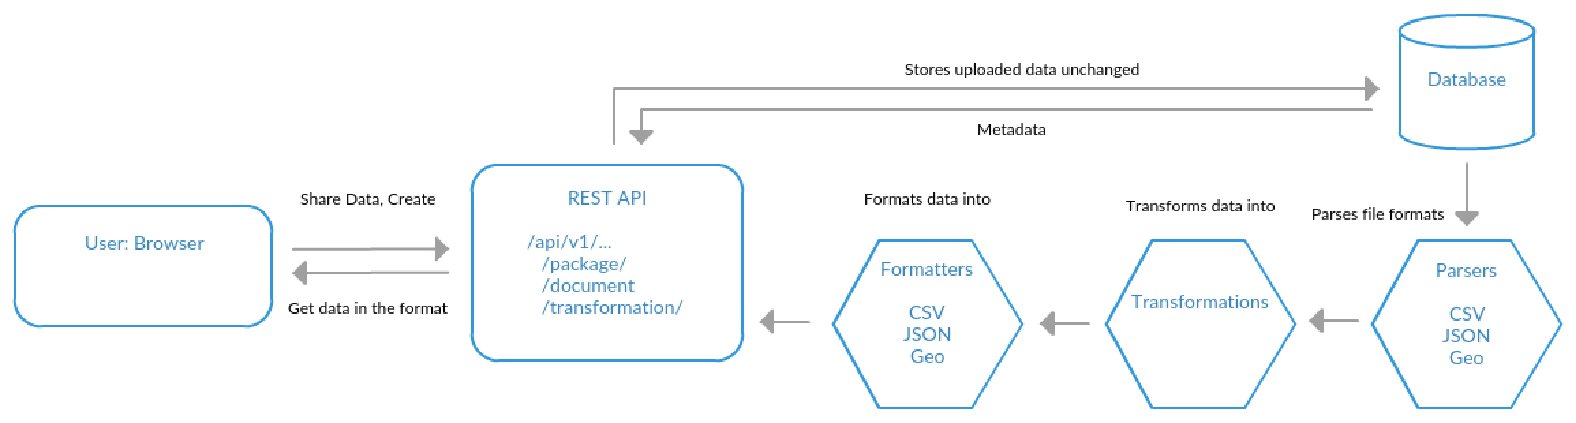
\includegraphics[width=\linewidth]{fig/ODH-Architecture-Overview}
    \caption{Grobe Architektur-Übersicht}
    \label{fig:pd:arch-overview}
\end{figure}

\subsection{Komponenten und Packages}
\cref{fig:pd:pypackages} erläutert die Package-Struktur und deren Inhalt der Python Module. Alle Python Module die sich im \path{plugins} Modul befinden, werden automatisch geladen. Darin befinden sich auch Beispiel-Plugins einer \acs{odhql}-Funktion sowie zur Erweiterung der Format-Unterstützung.

\begin{figure}[H]
    \centering
    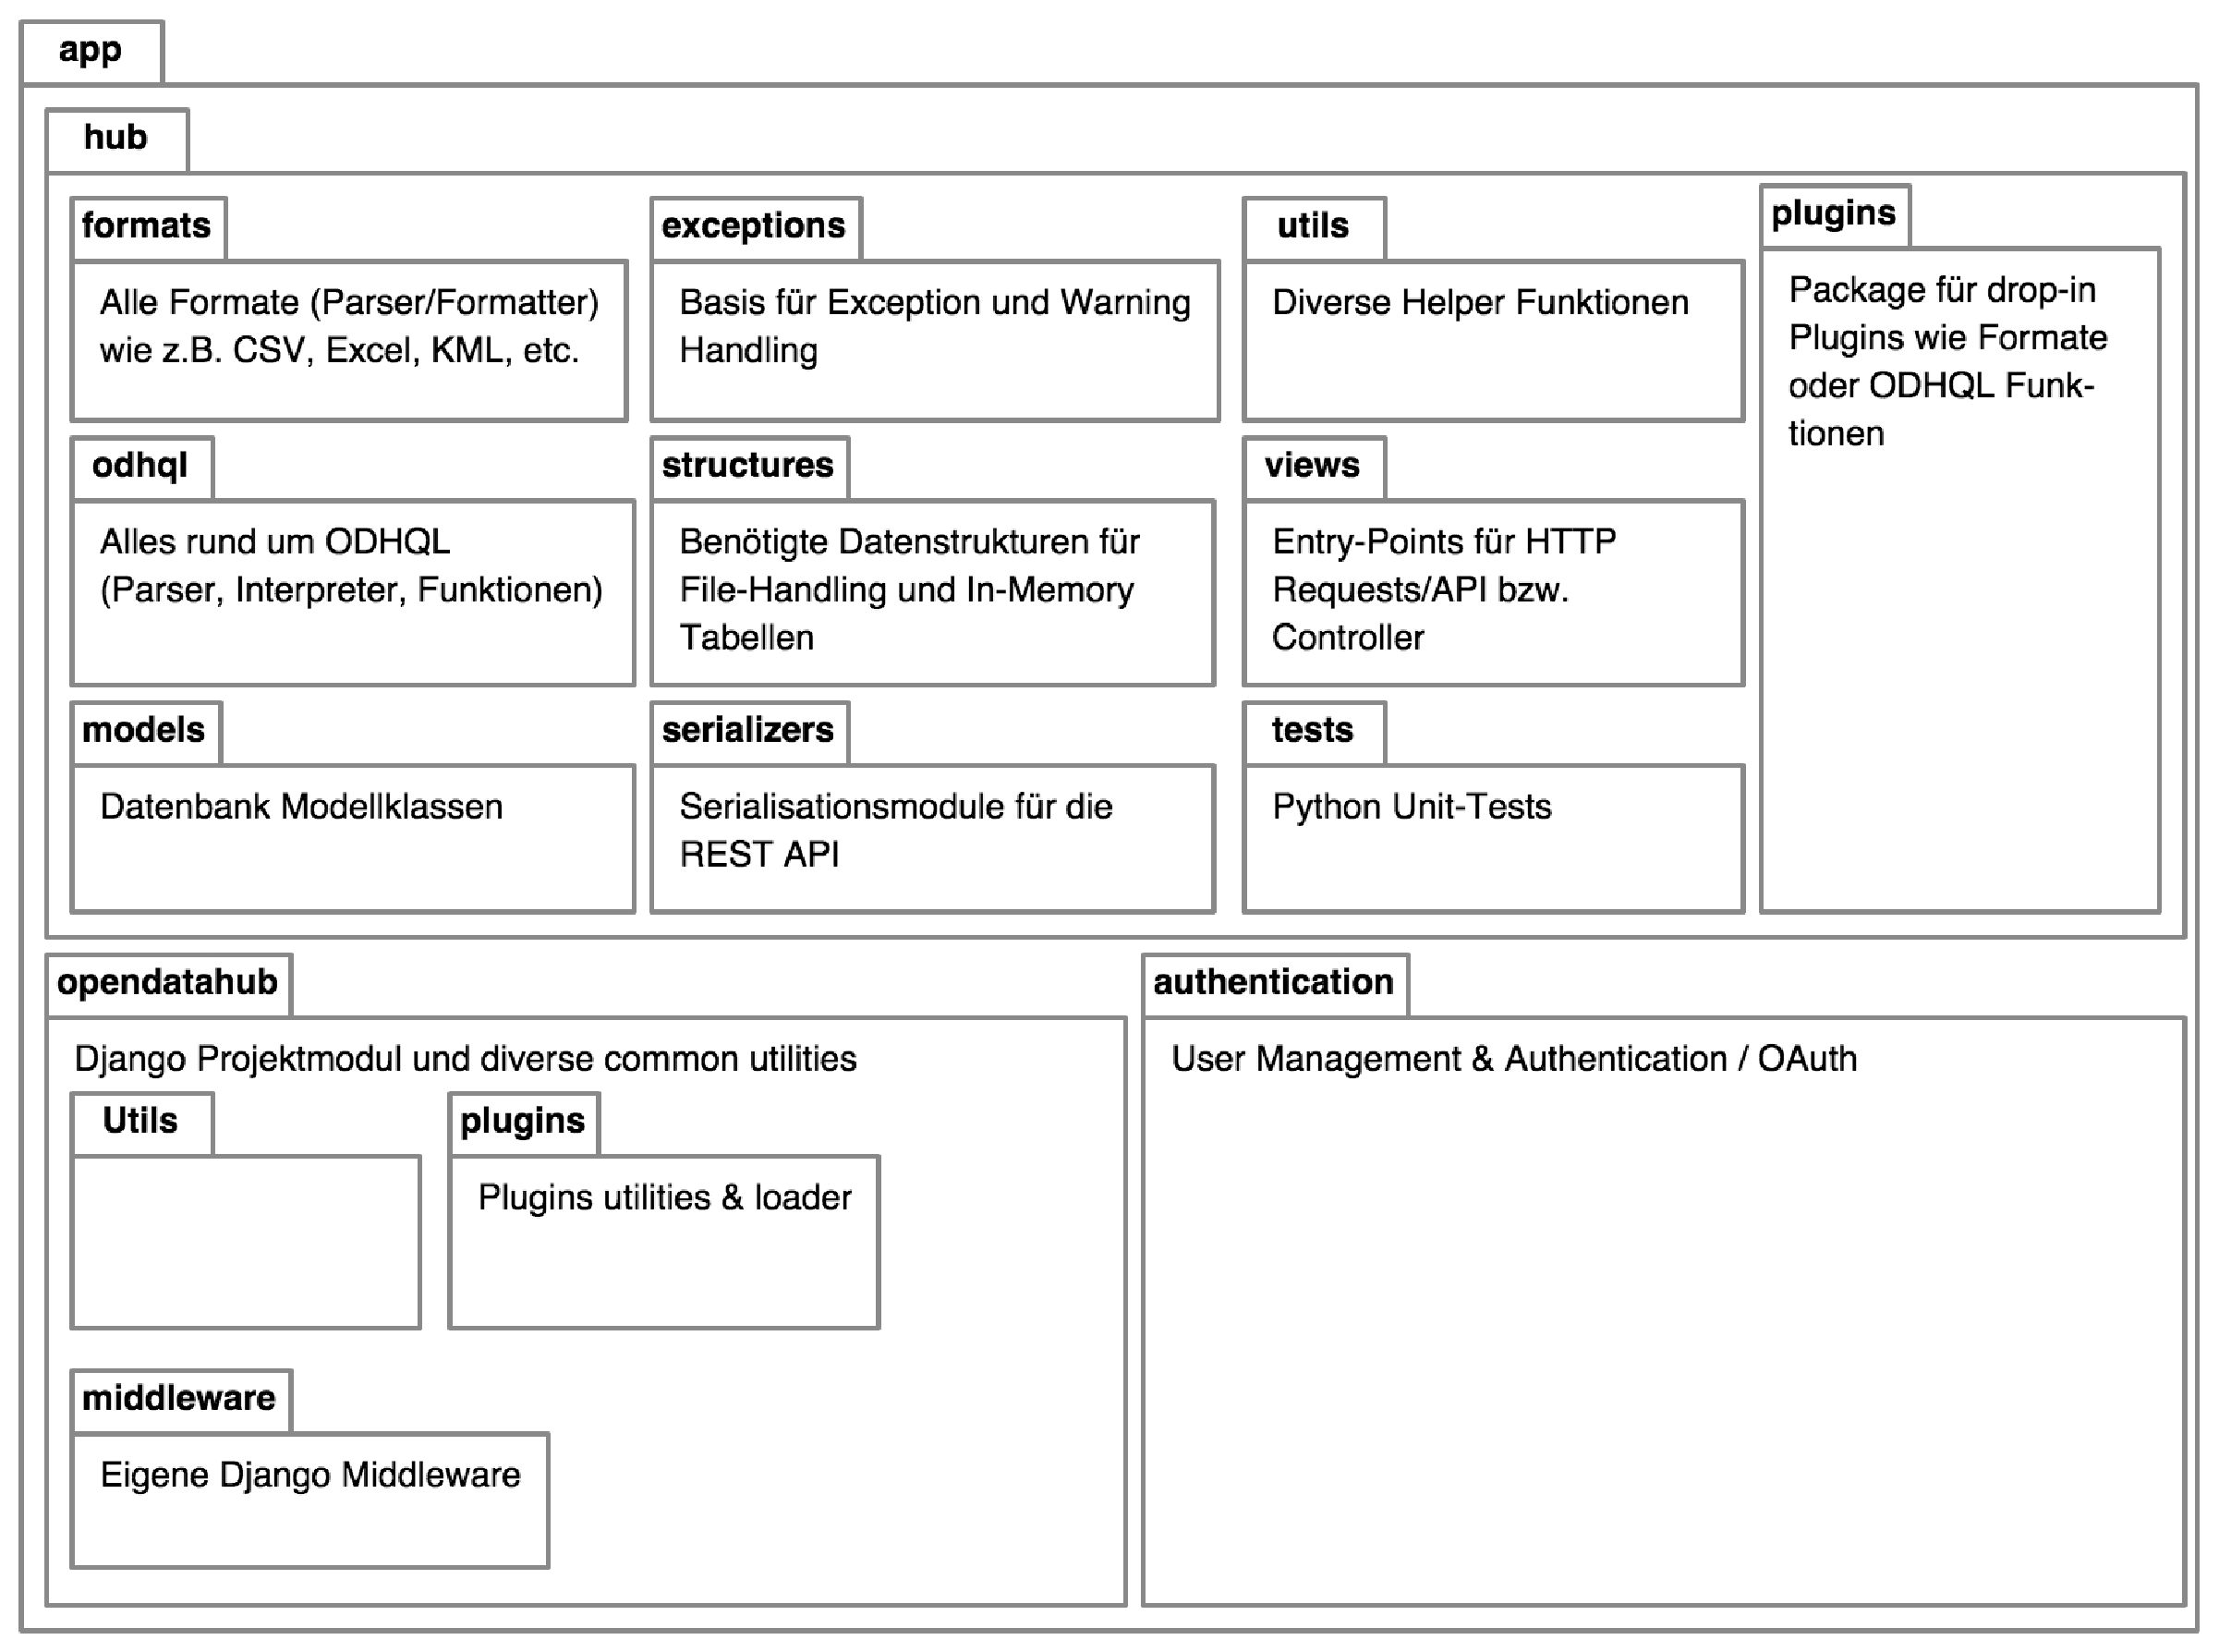
\includegraphics[width=\linewidth]{fig/packages}
    \caption{Python Packages}
    \label{fig:pd:pypackages}
\end{figure}

\subsection{Klassen}
Im folgenden werden einige besonders wichtige Klassen dargestellt.

\cref{fig:pd:modelclasses} zeigt die erstellten Django-Models\footnote{siehe auch \url{https://docs.djangoproject.com/en/1.8/topics/db/models/}}. Diese sind alle von \texttt{django.db.models.base.Model} abgeleitet.
\begin{figure}[H]
    \centering
    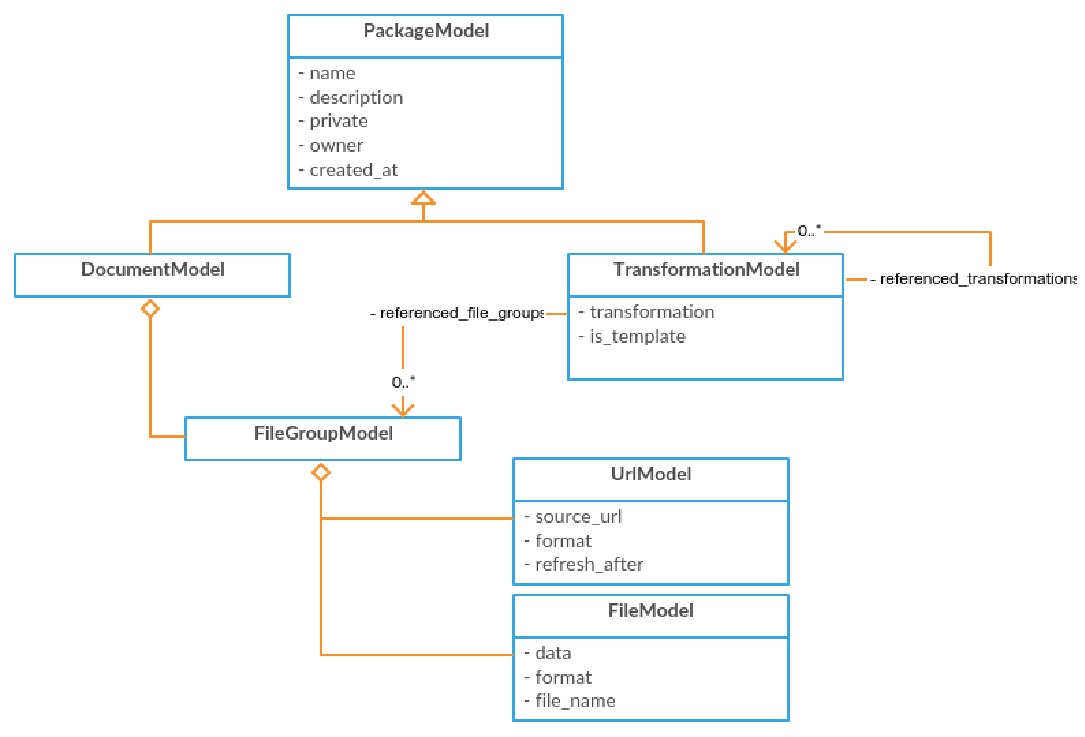
\includegraphics[width=\linewidth]{fig/model-classes}
    \caption{Django Models}
    \label{fig:pd:modelclasses}
\end{figure}
